\documentclass[paper=a4, fontsize=11pt]{scrartcl}
\usepackage[T1]{fontenc}
\usepackage{fourier}

\usepackage[english]{babel}															% English language/hyphenation
\usepackage[protrusion=true,expansion=true]{microtype}	
\usepackage{amsmath,amsfonts,amsthm} % Math packages
\usepackage[pdftex]{graphicx}	
\usepackage{url}
\usepackage{hyperref}


%%% Custom sectioning
\usepackage{sectsty}
\allsectionsfont{\centering \normalfont\scshape}
\usepackage{subfigure}
\usepackage{comment}


%%% Custom headers/footers (fancyhdr package)
\usepackage{fancyhdr}
\pagestyle{fancyplain}
\fancyhead{}											% No page header
\fancyfoot[L]{}											% Empty 
\fancyfoot[C]{}											% Empty
\fancyfoot[R]{\thepage}									% Pagenumbering
\renewcommand{\headrulewidth}{0pt}			% Remove header underlines
\renewcommand{\footrulewidth}{0pt}				% Remove footer underlines
\setlength{\headheight}{13.6pt}


%%% Equation and float numbering
%\numberwithin{equation}{section}		% Equationnumbering: section.eq#
%\numberwithin{figure}{section}			% Figurenumbering: section.fig#
%\numberwithin{table}{section}				% Tablenumbering: section.tab#


%%% Maketitle metadata
\newcommand{\horrule}[1]{\rule{\linewidth}{#1}} 	% Horizontal rule

\title{
		%\vspace{-1in} 	
		\usefont{OT1}{bch}{b}{n}
		\normalfont \normalsize \textsc{CS650 - Computer Vision} \\ [25pt]
		\horrule{0.5pt} \\[0.4cm]
		\huge Programming Lab 5 \\ Image Stitching \\
		\horrule{2pt} \\[0.5cm]
}
\author{
		\normalfont %\normalsize
        Tim Price \and Daqing Yi \\
}
%\date{}


%%% Begin document
\begin{document}
\maketitle

\begin{comment}
Step 1: Calculate Homography 
 high-contrast corners (Manual)
Step 2: Warp images
 backward mapping method (bilinear interpolation)
 
Extra credits:
(1) stitch the images by using a simple blending of them
(2) Use linear regression (more than four points)
(3) Use RANSAC (support bad point matches)
(4) Find points automatically using point detectors
\end{comment}

\begin{comment}
(1) GUI
Create GUI framework (DQ)
File loading (Tim)
Image displaying (DQ)
(2) Homography
Four point algorithm
(3) Warp
(3.1)Display a warped polygon
(3.2)Fill pixels using billinear interpolation
(4) Blending
(4.1) Average
(4.2) Weighted average
(5) Linear Regression
(6) RANSAC
\end{comment}

\section{Introduction}
%Tim
Stitching is a method used to merge multiple pictures of the same thing into a single large picture that encompasses everything all other pictures show.  
This is a very useful method in computer vision. 
However, the pictures often times have to be warped to fit each other as the perspective on the target object changes as the angle of the camera to that object changes.  
This lab focuses on warping various images of an object and stitching the images together to create a single large image of the object.

In this scenario, we used \emph{IMG\_1341.JPG} as a master image.
All other images in the set were compared to and warped to match the flow of this one.
The implementations are written in Python.
Pyqt is used for creating GUI for user operation.
CV2 (open CV) is used for reading image files into data arrays and display processed images in single test files.
Numpy is used for scientific operation, especially matrix calculation.

\section{Computing Homography}
%DQ

Homography is used to denote the transformation from one image plane to the other.
It is written as 
\begin{equation}
\label{eq:homography}
\begin{bmatrix}
x' \\
y' \\
1
\end{bmatrix}
\sim
\begin{bmatrix}
\tilde{x}' \\
\tilde{y}' \\
\tilde{w}'
\end{bmatrix}
=
\begin{bmatrix}
h_{00} & h_{01} & h_{02} \\
h_{10} & h_{11} & h_{12} \\
h_{20} & h_{21} & 1 
\end{bmatrix}
\begin{bmatrix}
x \\
y \\
1
\end{bmatrix}.
\end{equation}
By writing Equation \ref{eq:homography} as
\begin{equation}
\label{eq:homography_linear_form}
\begin{bmatrix}
x & y & 1 & 0 & 0 & 0 & -x'x & -x'y \\
0 & 0 & 0 & x & y & 1 & -y'x & -y'y
\end{bmatrix}
\begin{bmatrix}
h_{00} \\
h_{01} \\
h_{02} \\
h_{10} \\
h_{11} \\
h_{12} \\
h_{20} \\
h_{21} 
\end{bmatrix}
=
\begin{bmatrix}
x' \\ y'
\end{bmatrix},
\end{equation}
having four points (no three points in a line) is enough to calculate the homography. 
The implementation is in \emph{calcHomograph} method in \emph{ImageManager.py}.
In order to verify the correctness of the homography, the points are mapped into same image plane and the differences are compared.

Mapping \emph{IMG\_1342.JPG} to \emph{IMG\_1341.JPG} gets the homography using four-point algorithm as in Table \ref{tb:homograph:four_point}.
\begin{table}
\caption{Homography from \emph{IMG\_1342.JPG} to \emph{IMG\_1341.JPG} using Four-point algorithm}
\label{tb:homograph:four_point}
\begin{center}
\begin{tabular}{|c|c|c|}
	\hline
	9.77277130e-01 & -9.65971449e-02 &  8.45406980e+00\\
	\hline
	6.48954671e-03 &  8.70815189e-01 &  7.77927885e+02\\
	\hline
	7.65163108e-06 & -6.06586989e-05 &  1.00000000e+00\\
	\hline
\end{tabular}
\end{center}
\end{table}

\section{Warping the Images}
%Tim
Bilinear interpolation was used to warp the images.  
The homography matrix allows a point from the original image to be converted to the equivalent point on the target image.  
Since bilinear interpolation often works better going from the target to the original, I had to take the inverse of the homography matrix to do the calculation.  
All four corners on the original image were calculated using the homography matrix first to get the smallest and largest x and y points the new image would be.  
A new image was then created using these points for the size.  
Each point on the new image was then mapped to the original image and a bilinear interpolation of the point on that original image was used to determine the color of the new point.

Figure \ref{fig:warping} shows two images that were warped using this method to produce new images that could be used to stitch into \emph{IMG\_1341.JPG}.  



\begin{figure}[h]
\centering
\subfigure[Warp \emph{IMG\_1343.JPG} to the image plane of \emph{IMG\_1341.JPG}.]{
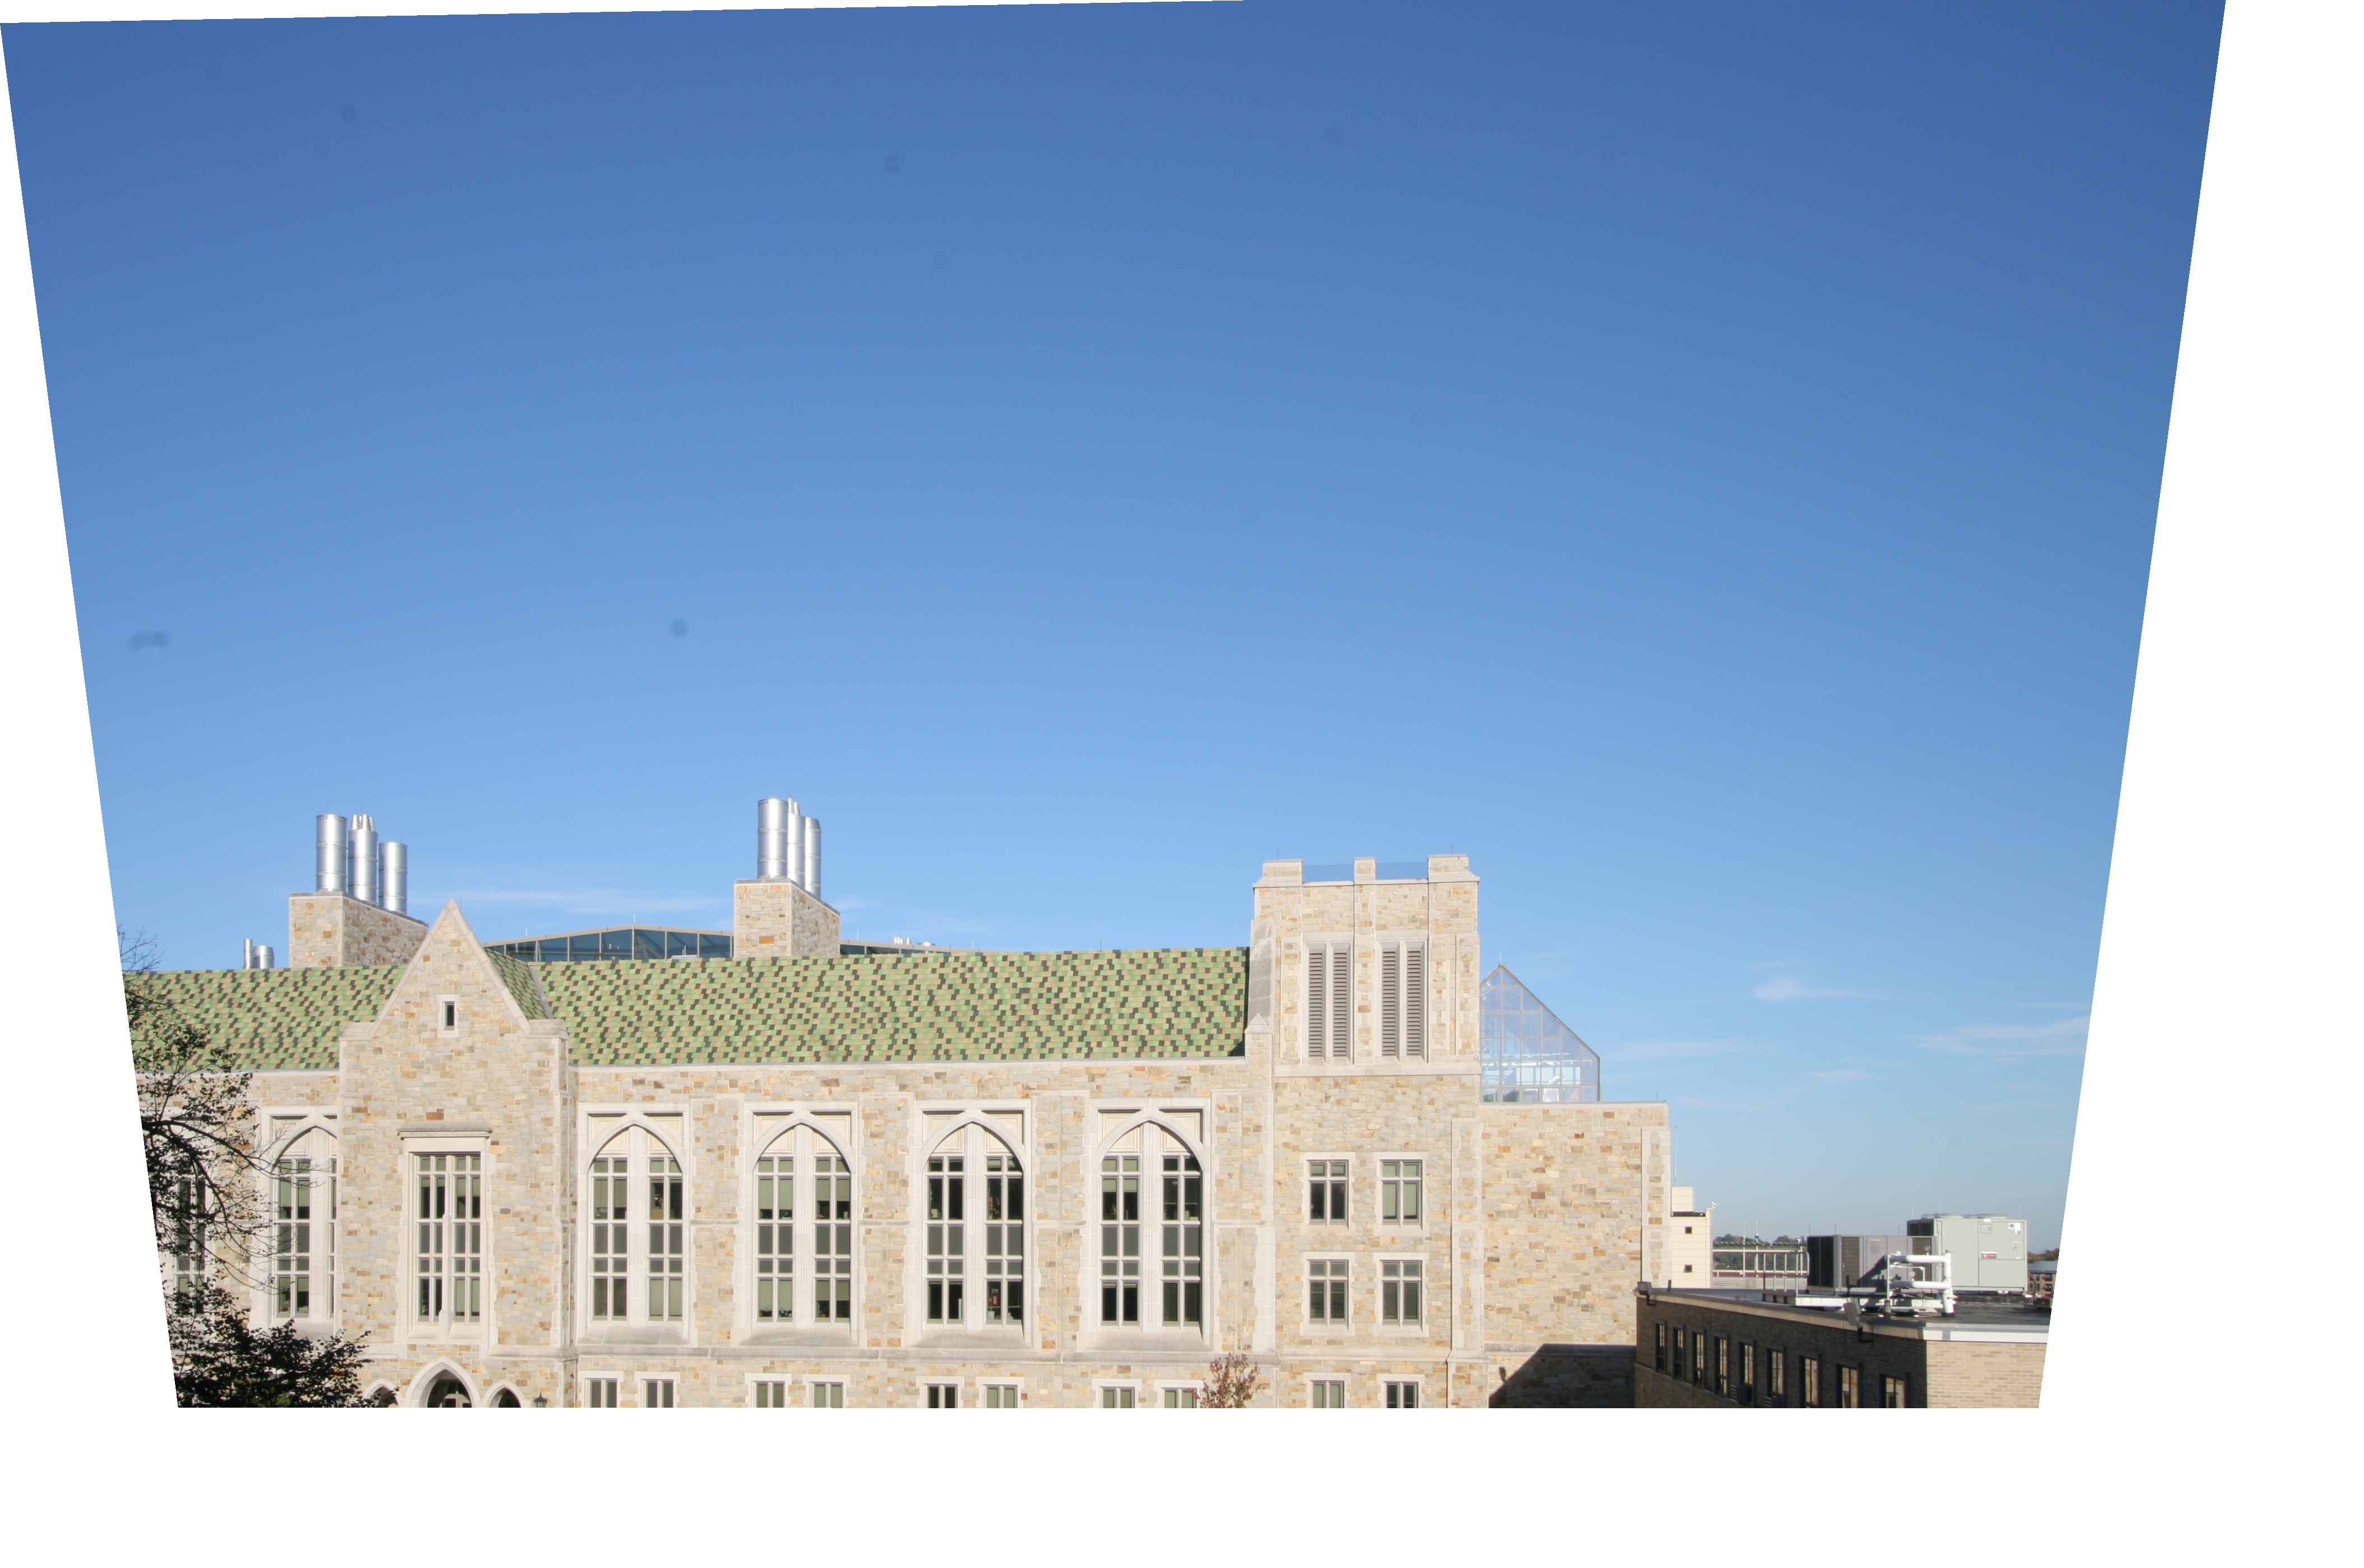
\includegraphics[width=.45\textwidth]{./figure/2_to_0.png} 
\label{fig:warping:01} } 
\subfigure[Warp \emph{IMG\_1345.JPG} to the image plane of \emph{IMG\_1341.JPG}.]{
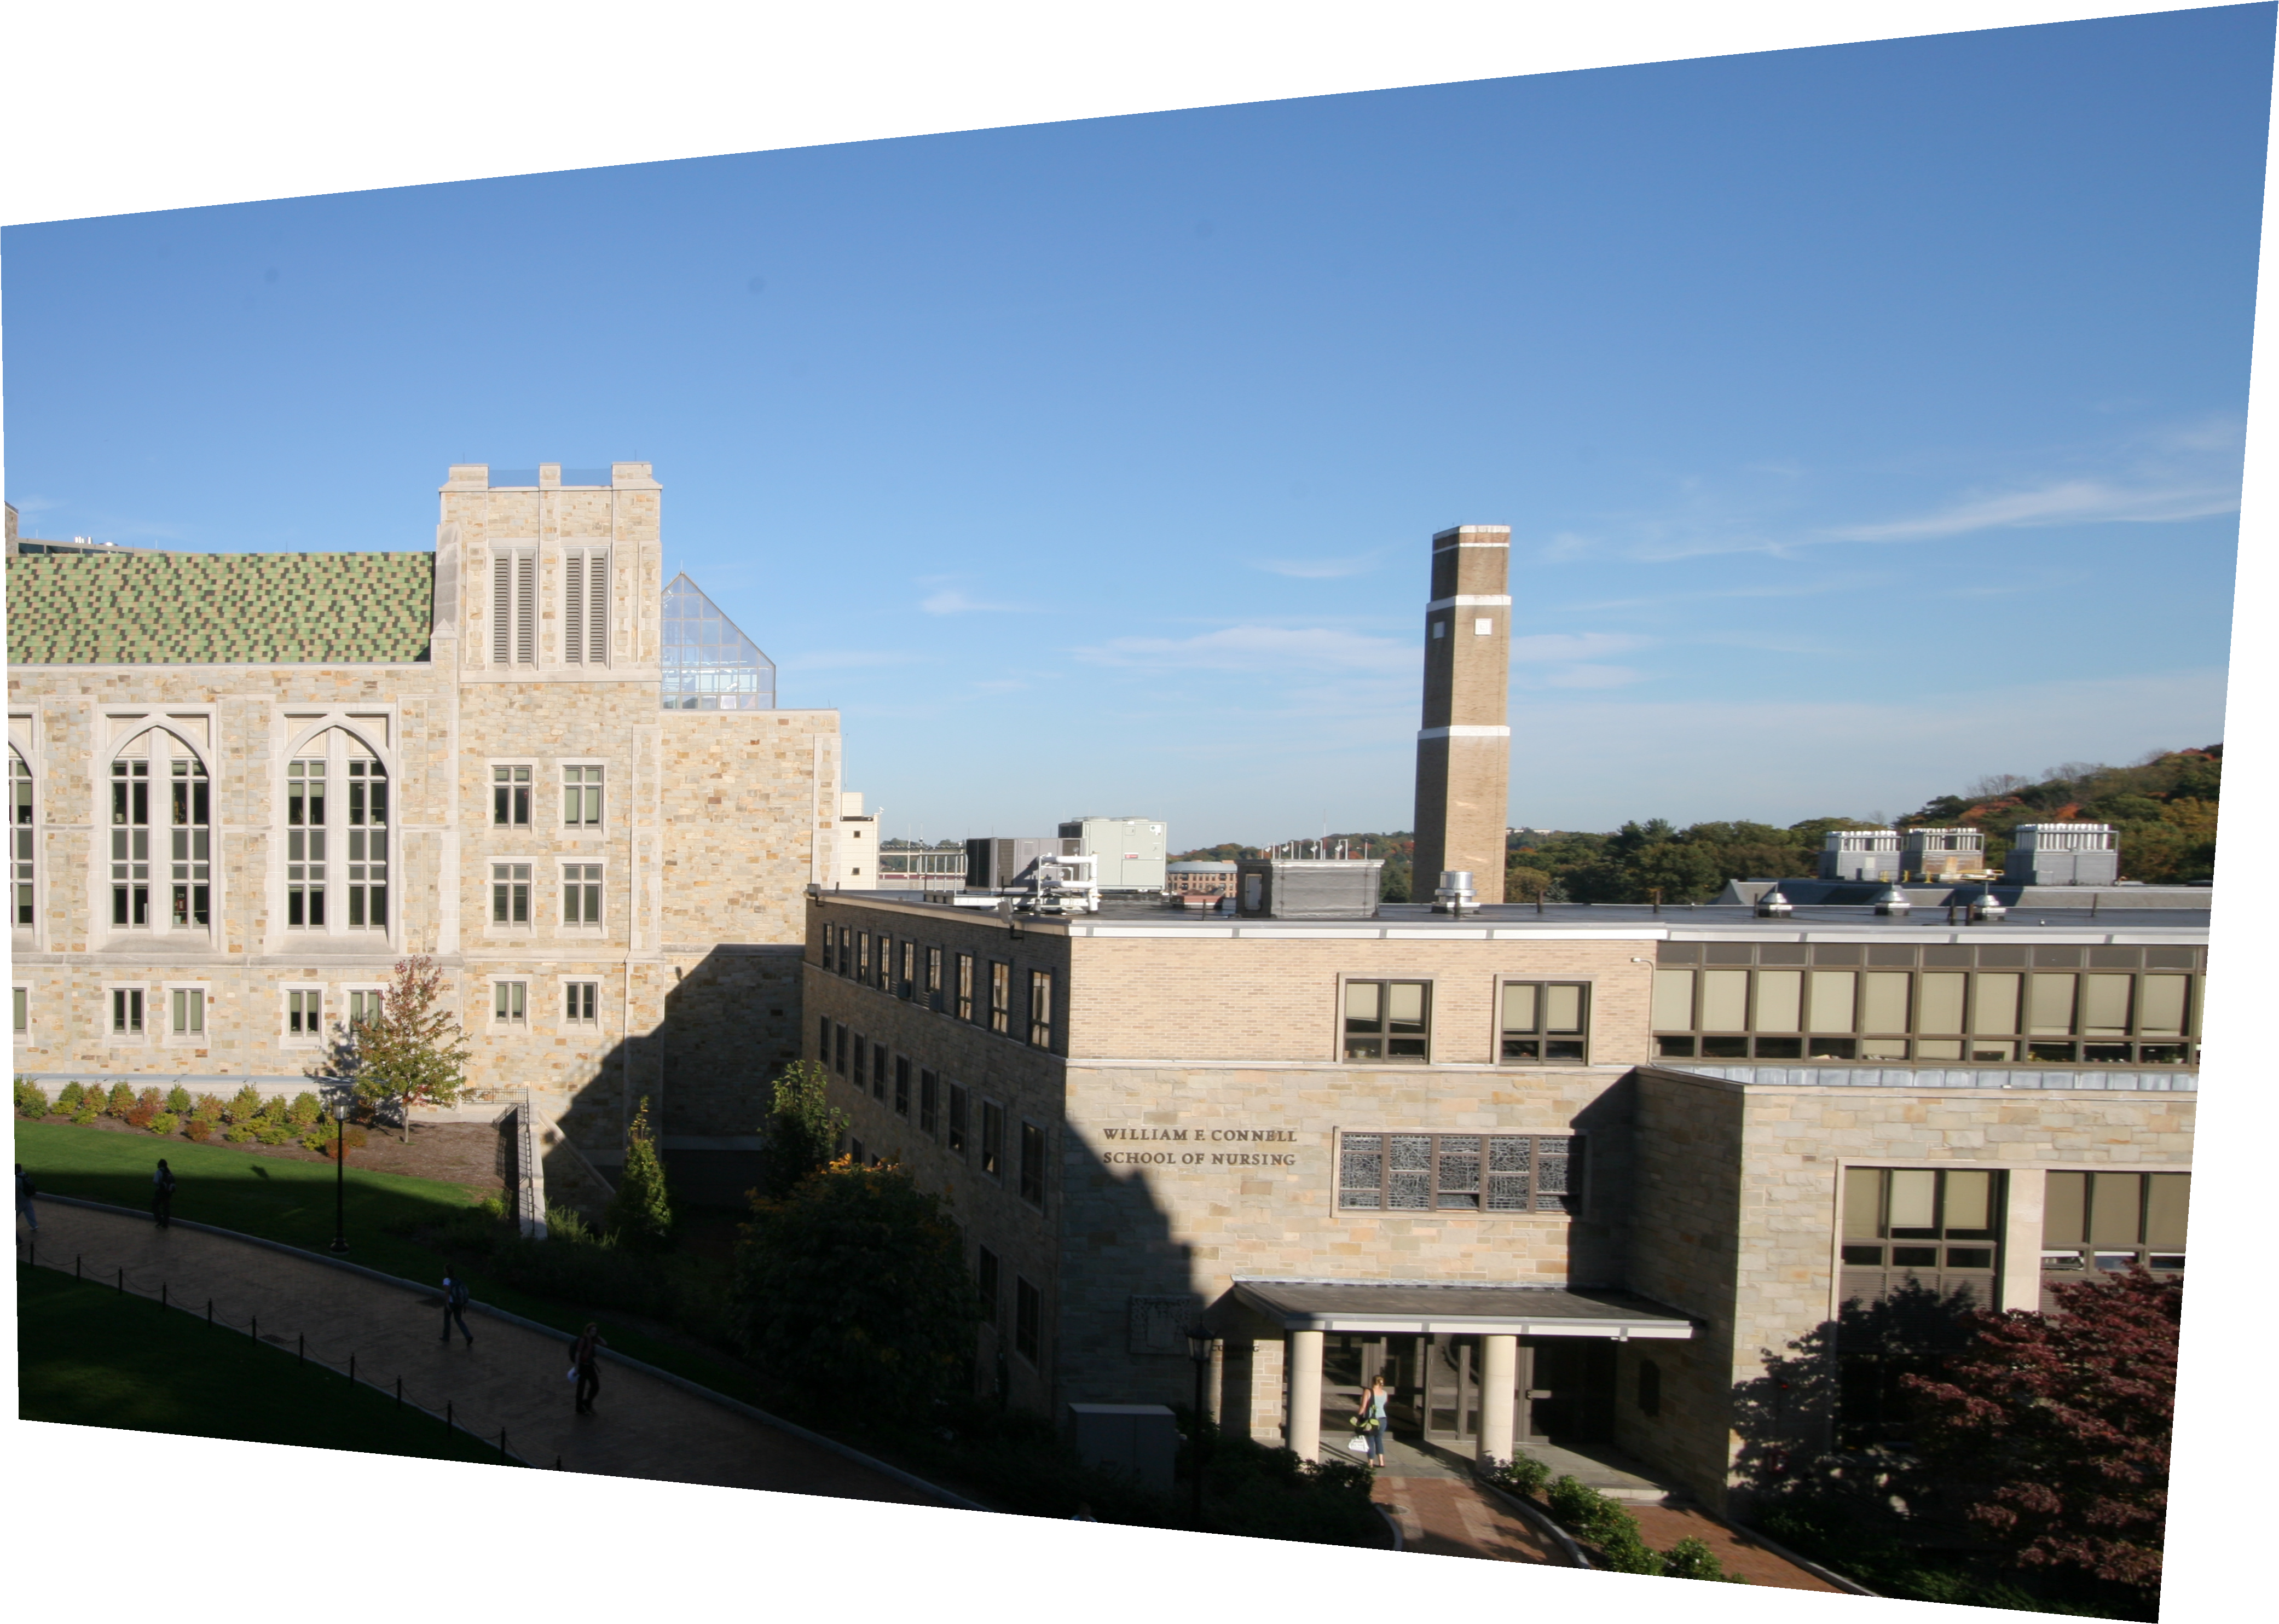
\includegraphics[width=.45\textwidth]{./figure/4_to_0.png} 
\label{fig:warping:02} } 
\caption{Image warping.}
\label{fig:warping}
\end{figure}

\section{Extra}

\subsection{Stitching the images}
%Tim
After the images are warped, they are stitched together.  
The new image is placed over the original one and a new image is created that encompasses both of them.  
This was then extended to run with all images in the set.  
In the original setup, the new image would be overlayed on top of the original one.  
However, we created a method that will average the all of the images together for each point to produce a blended image of all of the smaller ones put together.


\begin{figure}[h]
\centering
\subfigure[Blend \emph{IMG\_1342.JPG} with \emph{IMG\_1341.JPG}.]{
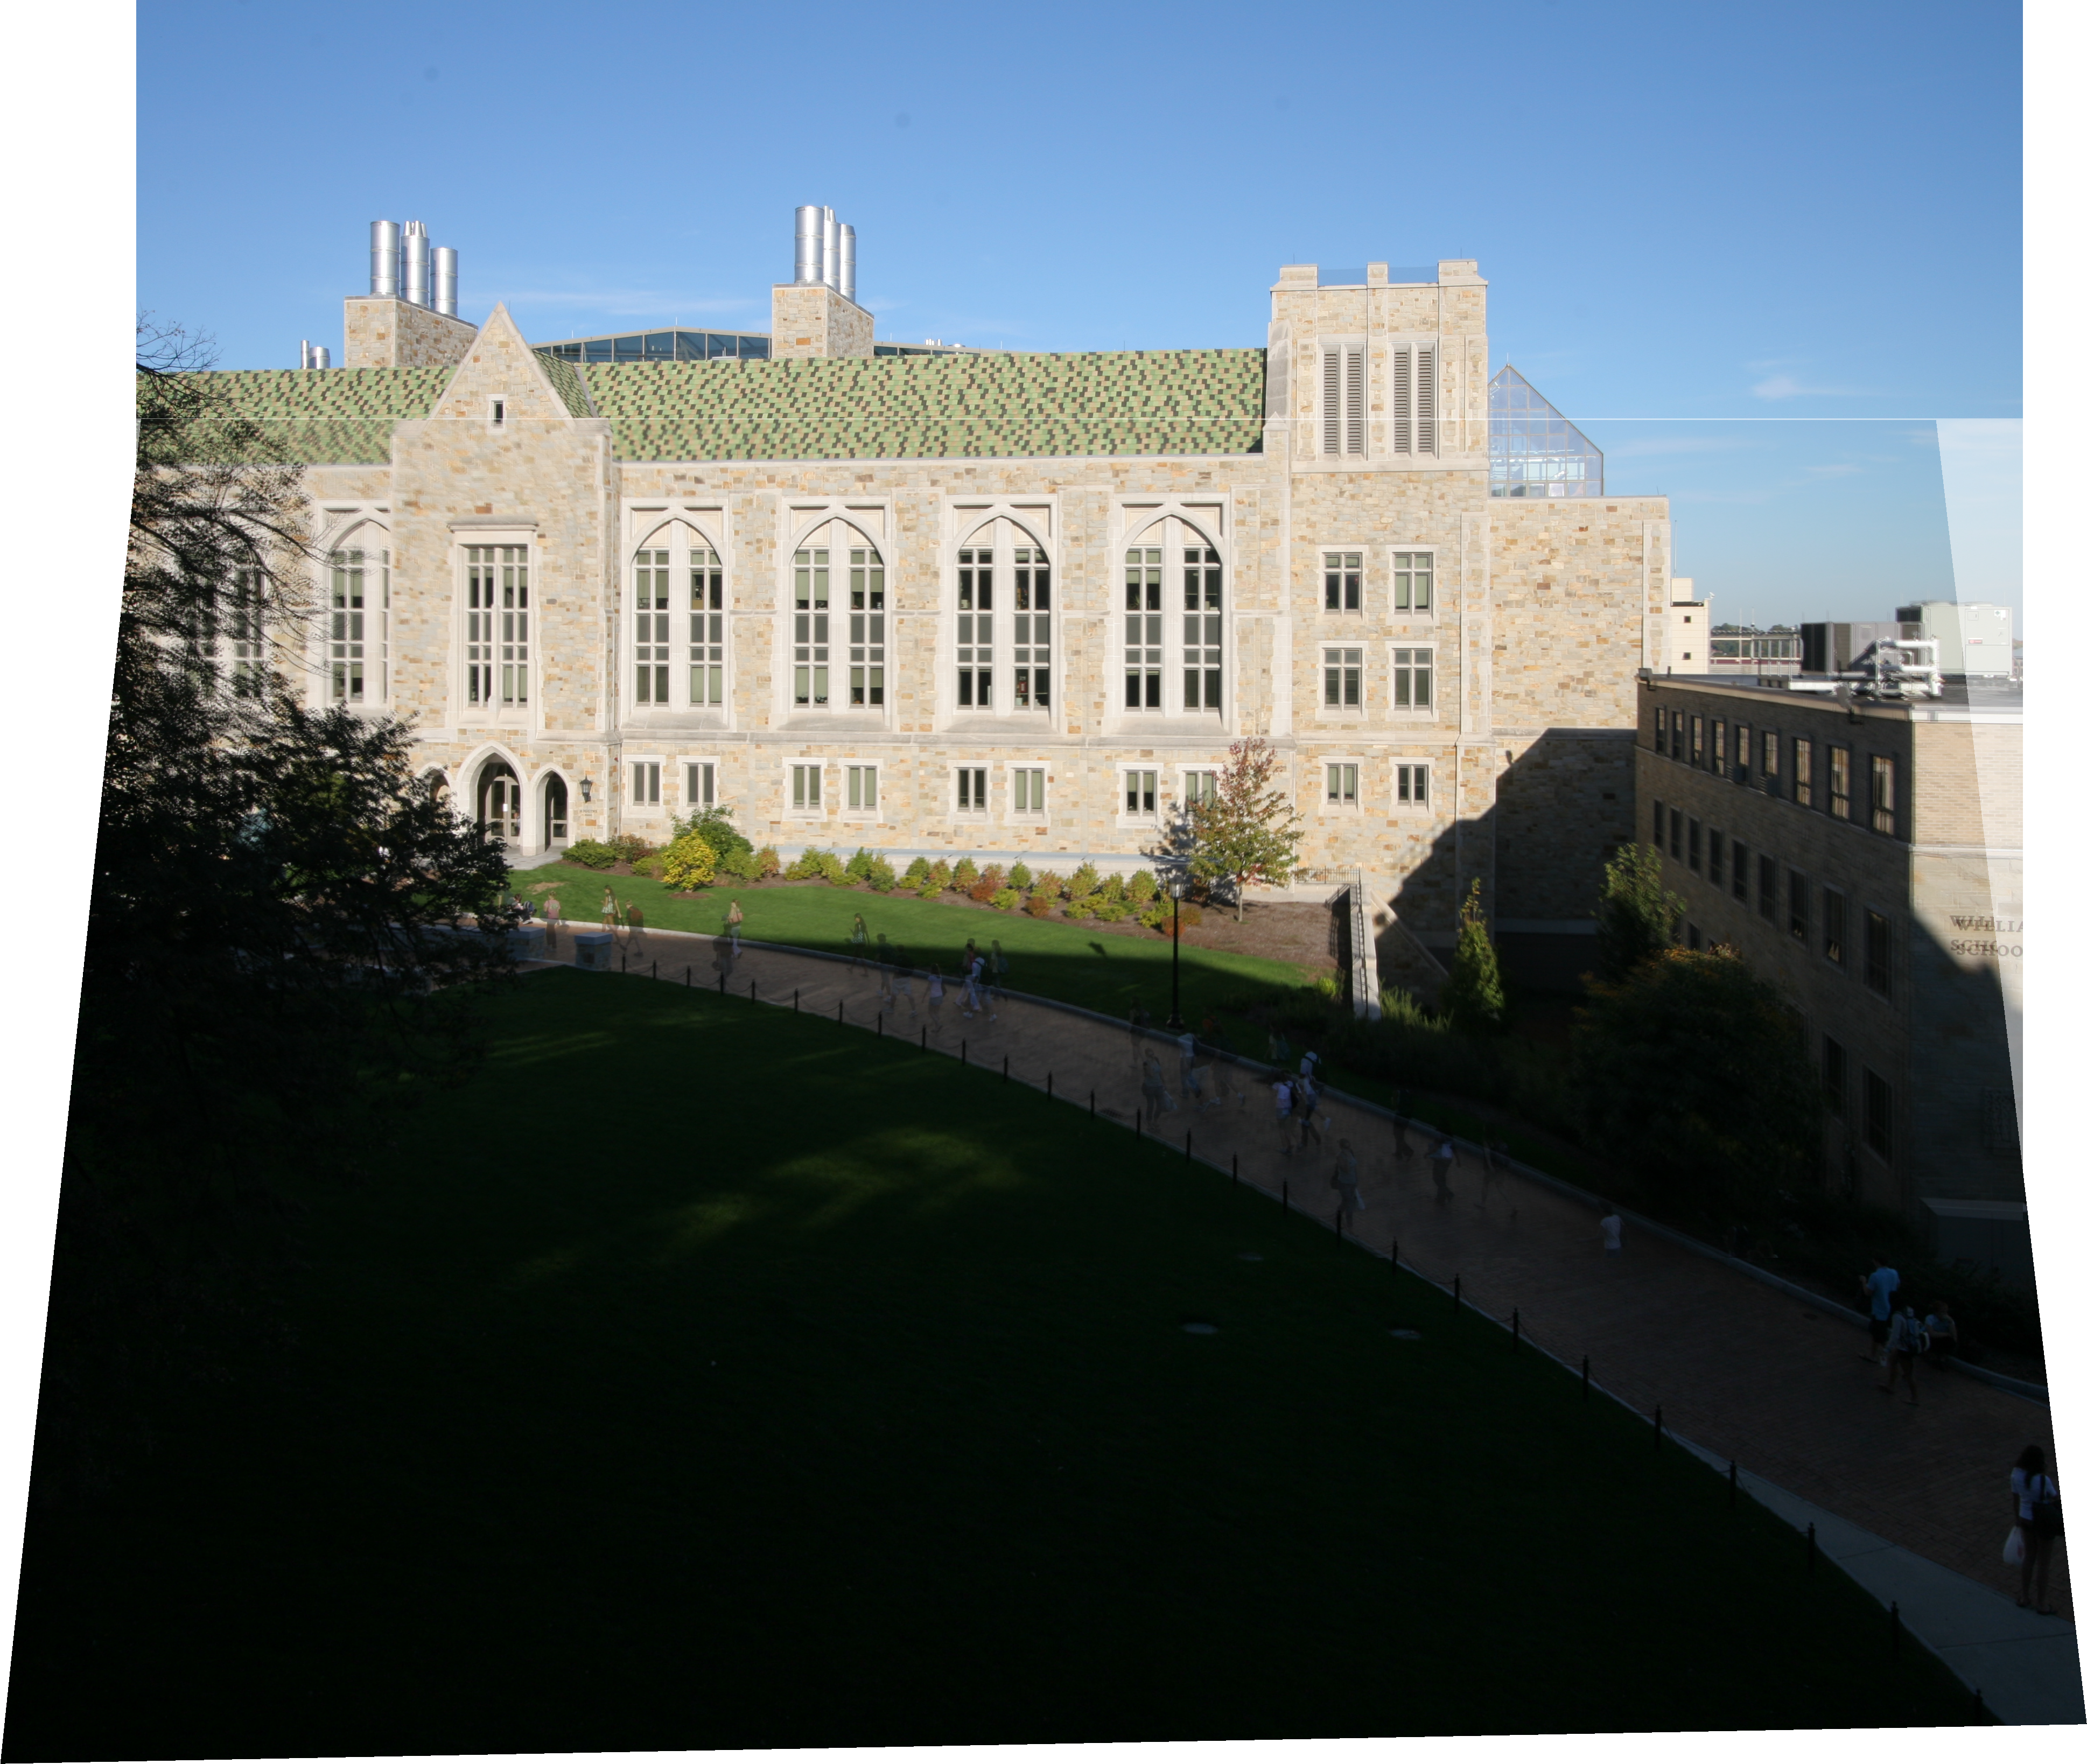
\includegraphics[width=.45\textwidth]{./figure/1_and_0.png} 
\label{fig:blending:01} } 
\subfigure[Blend \emph{IMG\_1344.JPG} with \emph{IMG\_1341.JPG}.]{
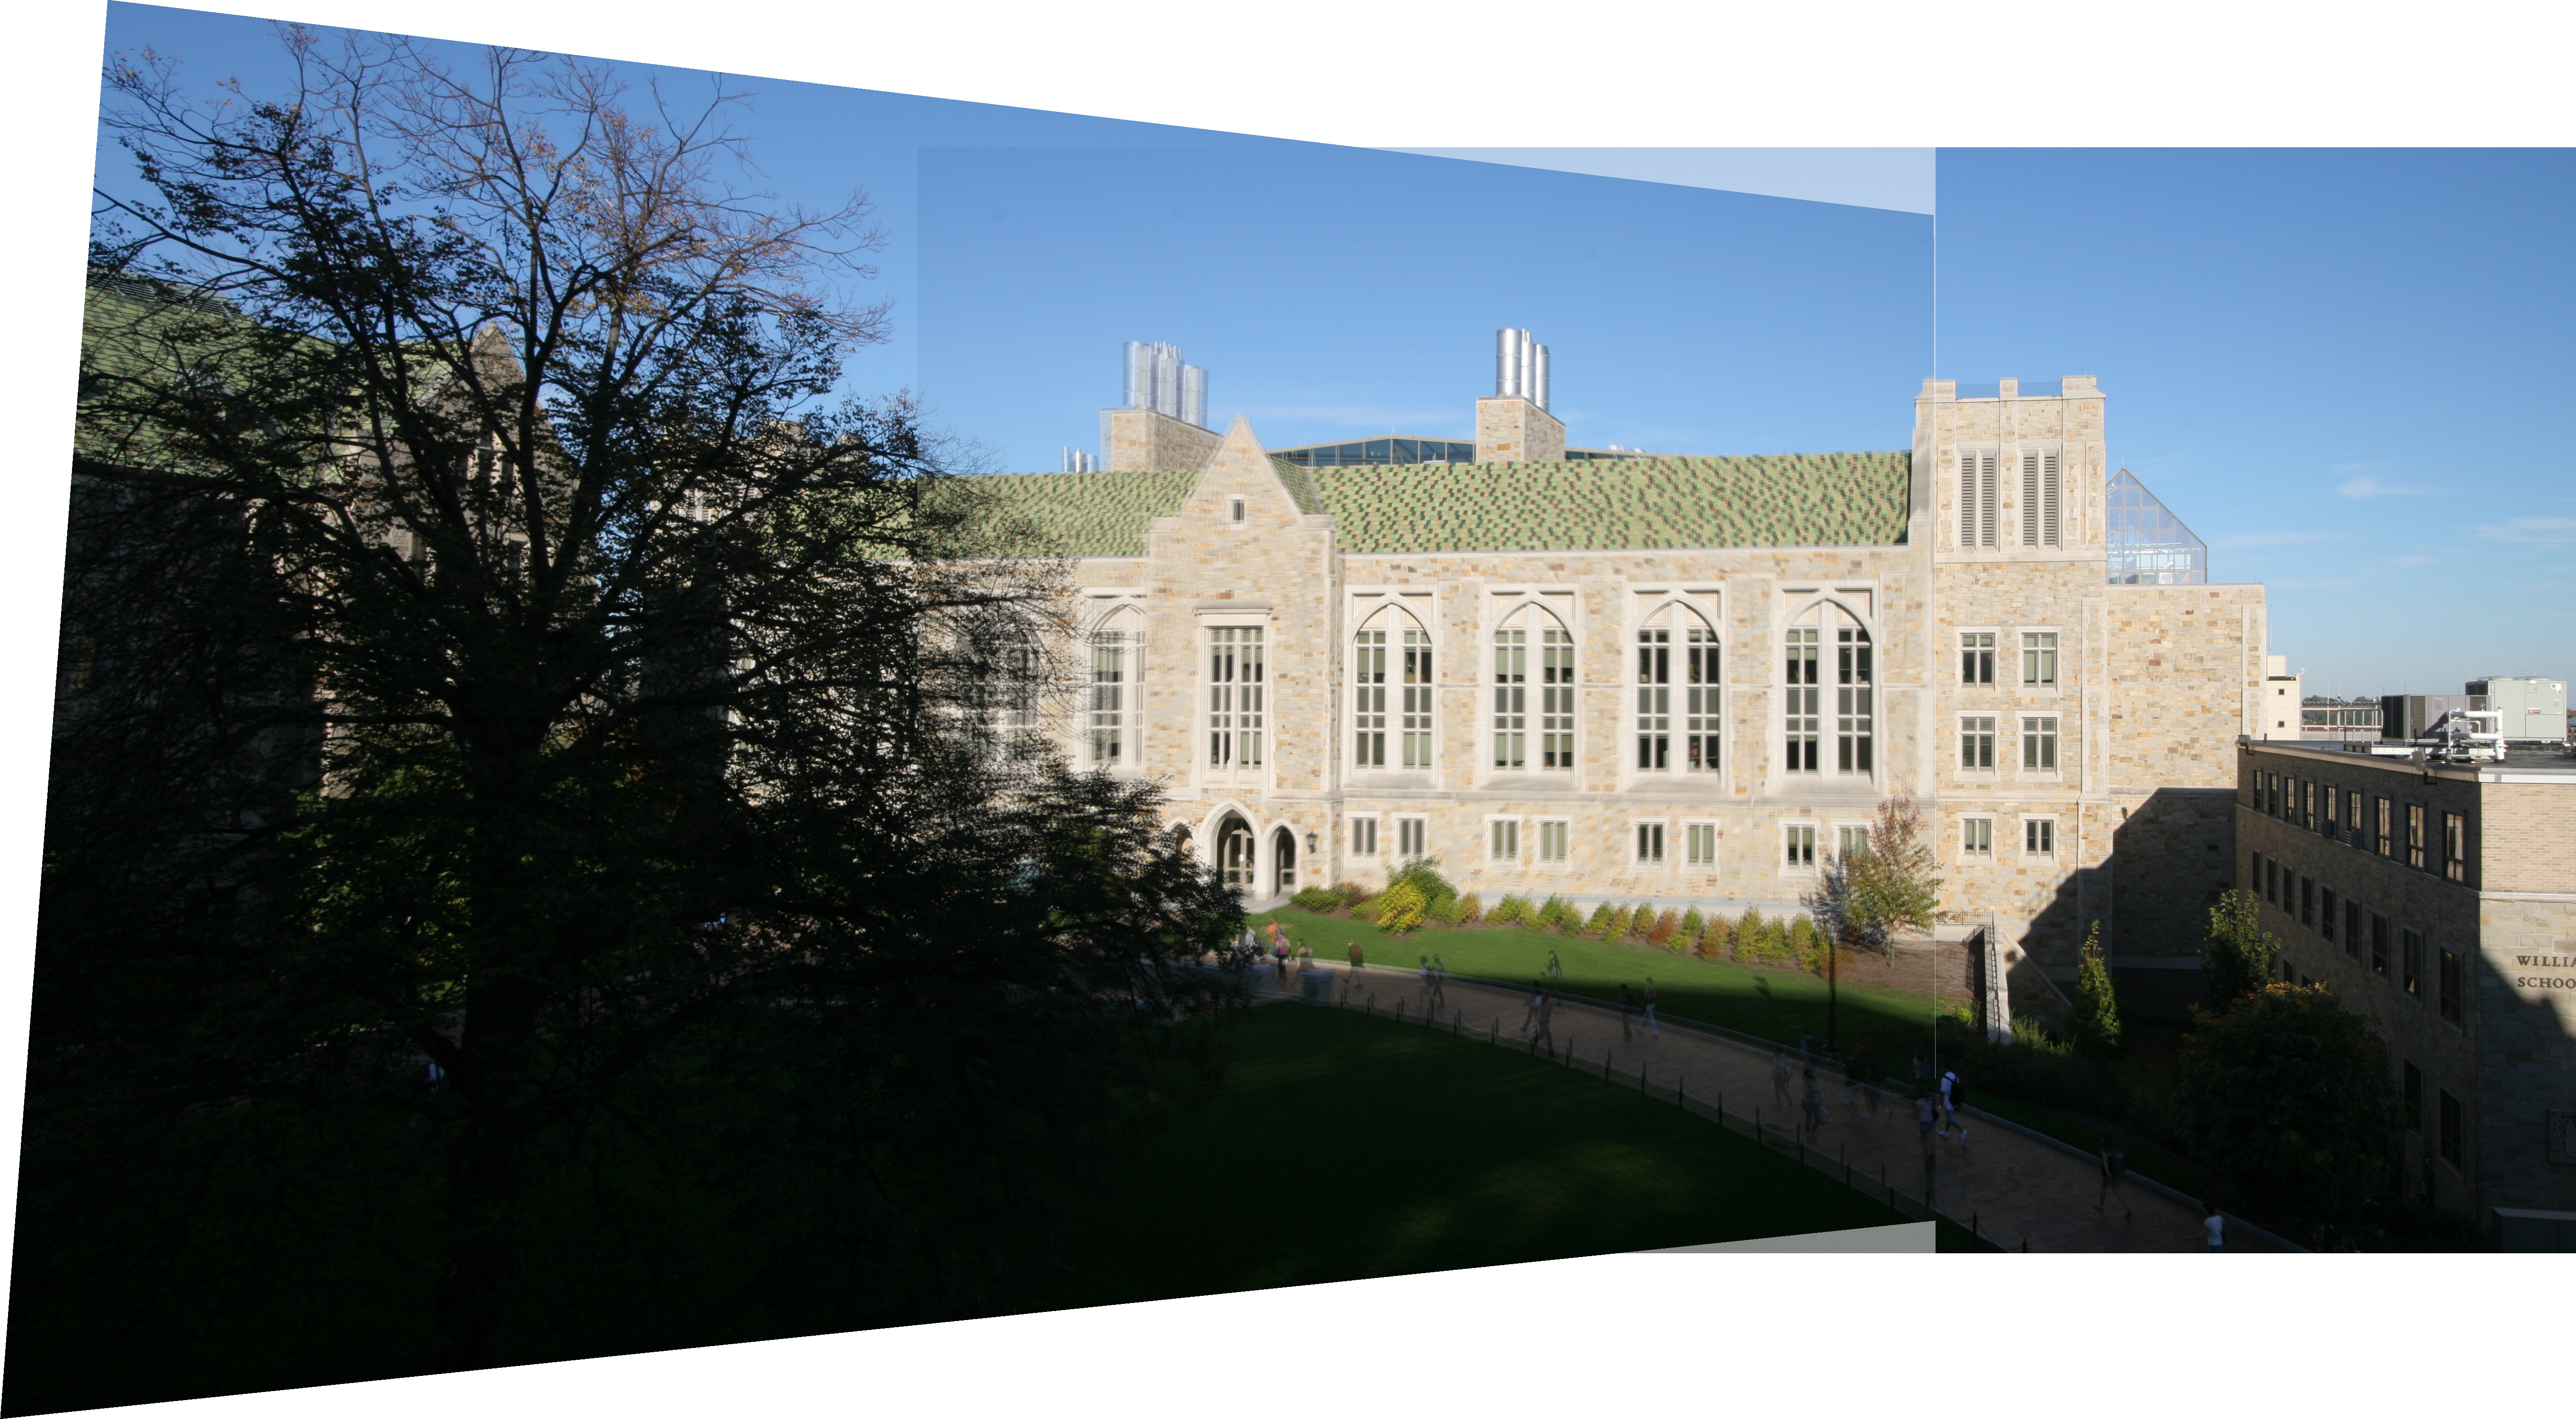
\includegraphics[width=.45\textwidth]{./figure/3_and_0.png} 
\label{fig:blending:02} } 
\caption{Image blending.}
\label{fig:blending}
\end{figure}

\begin{figure}[h]
\centering
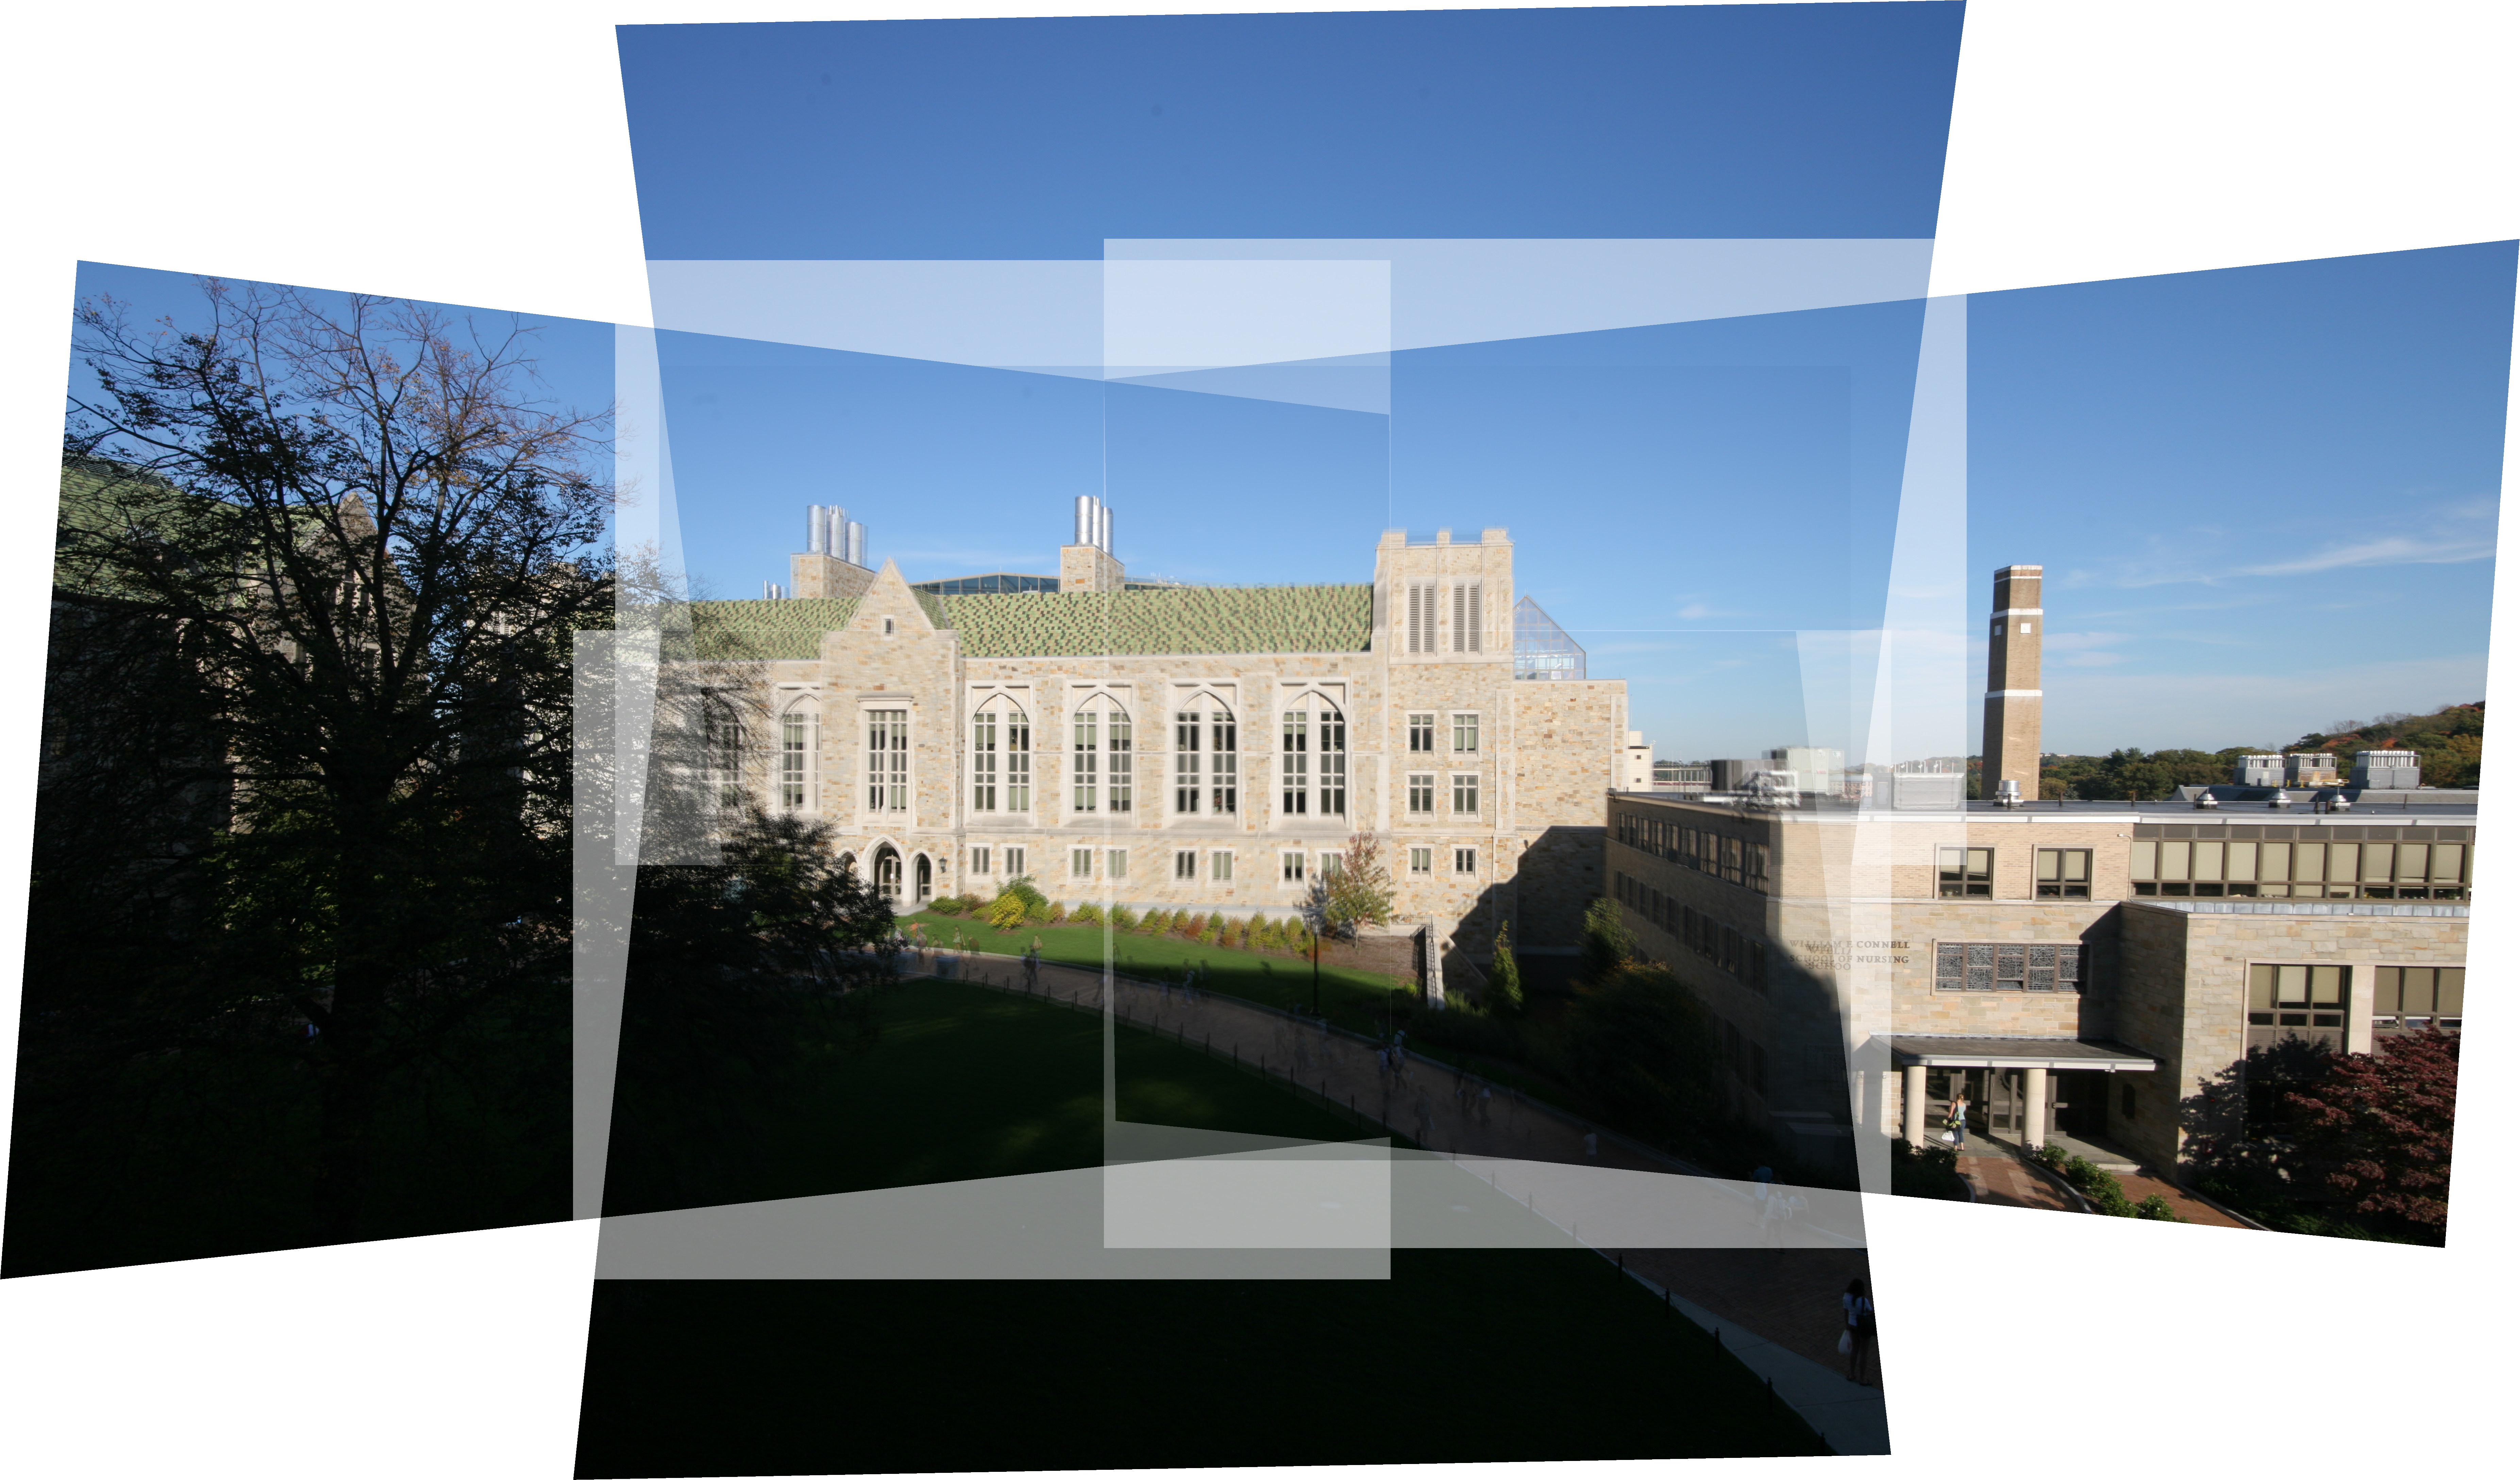
\includegraphics[width=\textwidth]{./figure/1_2_3_4_and_0.png} 
\caption{Stitched image.}
\label{fig:stitched_image}
\end{figure}

\subsection{Homograph Calculation using linear least squares}
%DQ

We also tested using linear least squares to calculate the homography.
The implementation is given in method \emph{calcHomographyByRegression} in \emph{ImageManager.py}.
It enables the calculation of homography using more than four points.
By expressing the homography as a linear model in Equation \eqref{eq:homography_linear_form},
we can viewed the problem as a linear regression problem. 
Define the objective as least square error, the problem can be solved using Matrix method.
Given
\begin{equation}
Y = X \beta
\end{equation}
the problem can be solved by
\begin{equation}
\beta = (X^{T} X)^{-1} X^{T} Y.
\end{equation}

Table \ref{tb:homograph:regression} gives an example using linear least squares.
Table \ref{tb:homograph:regression:error} gives the difference between the two homographies using four-point algorithm and using linear least squares respectively.
As the error is in a reasonable region, we believe the results from the regression are correct.

\begin{table}
\caption{Homography from \emph{IMG\_1342.JPG} to \emph{IMG\_1341.JPG} using regression}
\label{tb:homograph:regression}
\begin{center}
\begin{tabular}{|c|c|c|}
	\hline
	9.70610837e-01 & -1.00296632e-01 &  1.38072699e+01\\
	\hline
	4.59905259e-03 & 8.64781106e-01 &  7.79260185e+02\\
	\hline
	5.95562619e-06 & -6.28869645e-05 &  1.00000000e+00\\
	\hline
\end{tabular}
\end{center}
\end{table}

\begin{table}
\caption{Difference on homographies from \emph{IMG\_1342.JPG} to \emph{IMG\_1341.JPG} using four-point algorithm and using regression}
\label{tb:homograph:regression:error}
\begin{center}
\begin{tabular}{|c|c|c|}
	\hline
	6.66629234e-03 &  3.69948698e-03 & -5.35320014e+00\\
	\hline
	1.89049413e-03 &  6.03408229e-03 & -1.33229963e+00\\
	\hline
	1.69600489e-06 &  2.22826563e-06 &  0.00000000e+00\\
	\hline
\end{tabular}
\end{center}
\end{table}


\subsection{RANSAC}
%Tim
We developed a RANSAC algorithm to filter out good points from bad points when choosing the best set of points to use.  We fed it a set of points that have roughly 50\% good points.  We need 4 points to fit the model and taking a random sampling 80 times.  Using this information we determined that we had a 99.43 percent chance of getting a good set of data.

$$1-(1-0.5^4)^80$$
$$=99.43\%$$

Using this method and comparing it to the correct values, we got values very similar to the real set.  The following tables are the homographic values calculated comparing the first two pictures.
The homography using a known good set of points is shown above in Table \ref{tb:homograph:four_point}.
The calculated homography from RANSAC is given in Table \ref{tb:homograph:ransac}.
The difference between the two calculated homographies are given in Table \ref{tb:homograph:ransac:error}.
It shows that the error is in a reasonable region.

\begin{table}
\caption{Difference on homographies from \emph{IMG\_1342.JPG} to \emph{IMG\_1341.JPG} using four-point algorithm and using RANSAC}
\label{tb:homograph:ransac}
\begin{center}
\begin{tabular}{|c|c|c|}
\hline
9.83527679e-01 & -8.65639636e-02 &  3.36260667e+00\\
\hline
7.77270728e-03 &  8.87926310e-01 &  7.76424436e+02\\
\hline
8.92823558e-06 & -5.04489027e-05 &  1.00000000e+00\\
\hline
\end{tabular}
\end{center}
\end{table}


\begin{table}
\caption{Difference on homographies from \emph{IMG\_1342.JPG} to \emph{IMG\_1341.JPG} using four-point algorithm and using RANSAC}
\label{tb:homograph:ransac:error}
\begin{center}
\begin{tabular}{|c|c|c|}
\hline
6.25054914e-03 &  1.00331813e-02 & -5.09146313e+00\\
\hline
1.28316056e-03 &  1.71111209e-02 & -1.50344898e+00\\
\hline
1.27660450e-06 &  1.02097962e-05 &  0.00000000e+00\\
\hline
\end{tabular}
\end{center}
\end{table}

As can be seen, the error is very small from the two calculated homographies.  This shows that the RANSAC algorithm can produce good results from a set of noisy data.

\subsection{Automatic point detection}
%DQ
In order to calculate homography automatically, it is expected that the feature points are extracted automatically and prematched roughly.
Then the RANSAC could run over the prematched feature points in two images.

\subsubsection{Harris corner detector}

Harris corner detector is chosen to detect the feature points.
The implementation is in \emph{HarrisCornerDetector.py}.
The direction changes of the intensity is used for determining whether a pixel is a corner point.
The calculation follows a simplified equivalence, which is
\begin{equation}
W(x,y) = 
\begin{bmatrix}
W_{x2}(x,y) & W_{xy}(x,y) \\
W_{xy}(x,y) & W_{y2}(x,y),
\end{bmatrix} \\,
\end{equation}
$ W_{x2} = G(I_{x2}) $, $ W_{xy} = G(I_{x2}) $ and $ W_{y2} = G(I_{y2}) $.
$ G $ is Gaussian filter, $ I_{x2} $, $ I_{xy} $ and $ I_{y2} $ are obtained from image derivatives.
A local maximum is applied to detect the peaks in $ Det(W) / tr(W) $ as the corners.
The result of an example is given in Figure \ref{fig:corner_detection}.

\begin{figure}[h]
\centering
\includegraphics[width=.8\textwidth]{./figure/IMG_1341_hcd.jpg} 
\caption{Apply Harris corner detector to \emph{IMG\_1341.JPG}.}
\label{fig:corner_detection}
\end{figure}

\subsubsection{Prematch - Normalized Cross-Correlation}

\textbf{Normalized Cross-Correlation} is used to measure the similarities of two points when doing prematch.
It is defined as 
\begin{equation}
\mbox{ncc} = \frac{1}{n} \sum_{x, y} \frac{(I_{1}(x,y)-\bar{I}_{1})(I_{2}(x,y)-\bar{I}_{2})}{\sigma_{1}\sigma_{2}},
\end{equation}
in which $ \bar{I} $ is the mean and $ \sigma $ is the standard deviation.
When finding the matched points in Image 1 and Image 2, each point in Image 1 will take a point in Image 2 that has the biggest similarity (NCC) as a matched point in Image 2.
Figure \ref{fig:matching} gives an example of the matched points found in between \emph{IMG\_1341.JPG} and \emph{IMG\_1343.JPG}. 
Random colors are generated for each matched pair. 
The two points shared same color means they are paired as matched points.
We can see that there are some good matched points and some wrong matched points in Figure \ref{fig:matching}.

\begin{figure}[h]
	\centering
	\subfigure[Matched points in \emph{IMG\_1341.JPG}.]{
		\includegraphics[width=.8\textwidth]{./figure/IMG_1341_l.jpg} 
		\label{fig:matching:01} }
	\subfigure[Matched points in \emph{IMG\_1343.JPG}.]{
		\includegraphics[width=.8\textwidth]{./figure/IMG_1343_l.jpg} 
		\label{fig:matching:02} } 
	\caption{Points matching.}
	\label{fig:matching}
\end{figure}


\subsubsection{Applying RANSAC}
The RANSAC algorithm works for finding a set of good points to use as the homography points.
It can go through and produce a correct set from a lot of noisy points.
Table \ref{tb:homograph:auto_ransac} gives an example of the homography calculated using auto-RANSAC.
The difference with the result in Table \ref{tb:homograph:four_point} is given in Table \ref{tb:homograph:auto_ransac:error}.

\begin{table}
	\caption{Homography from \emph{IMG\_1342.JPG} to \emph{IMG\_1341.JPG} using auto-RANSAC.}
	\label{tb:homograph:auto_ransac}
	\begin{center}
		\begin{tabular}{|c|c|c|}
			\hline
			9.98712500e-01 & 7.71507381e-02 & -7.71480682e+01\\
			\hline
			-6.85093282e-03 &  9.53200118e-01 &  7.91061747e+02\\
			\hline
			-4.56872328e-07 &  1.64312878e-05 &  1.00000000e+00\\
			\hline
		\end{tabular}
	\end{center}
\end{table}

\begin{table}
	\caption{Differencce on homographies from \emph{IMG\_1342.JPG} to \emph{IMG\_1341.JPG} using four-point algorithm and using auto-RANSAC.}
	\label{tb:homograph:auto_ransac:error}
	\begin{center}
		\begin{tabular}{|c|c|c|}
			\hline
			2.14353706e-02 &  1.73747883e-01 &  -8.56021380e+01\\
			\hline
			-1.33404795e-02 &  8.23849289e-02 &  1.31338616e+01\\
			\hline
			-8.10850341e-06 &  7.70899867e-05 &  0.00000000e+00\\
			\hline
		\end{tabular}
	\end{center}
\end{table}

\section{Conclusion}
%This was a difficult but fun project. 
%Image stitching has a lot of benefits to producing a set of images together into a single one that has a lot more information than the others do.
%The most difficult portion was the automatic point detection.
%While we were able to get the RANSAC function working and we were able to find points that would work, matching them up was difficult.
%We ended up using a built in SIFT function to match the point which produced good results for the automatic point detection.  

\begin{itemize}
\item A great portion of time is spent in generating good matching points.
The parameter selection can influence the matching results significantly.
In this lab, because normalized cross correlation is used to measure the similarity, the window size can greatly impact the sensitivity of matching.
\item A strict consensus requirements for the consensus set reduces the number of samples for regression but guarantees the quality.
\end{itemize}


\bibliography{reference}
\bibliographystyle{plain}

\end{document}